\newpage
\changeindent{0cm}
\section{要素技術と 4 コマ漫画に関する従来研究}
\changeindent{2cm}

本章では,本研究に関連する要素技術について説明する. また, 4 コマ漫画に関する従来研究について概説する.

\changeindent{0cm}
\subsection{自然言語処理に関する要素技術}
\changeindent{2cm}

自然言語の単語や文を計算機上で表現するための分散表現獲得手法について説明する.

\changeindent{0cm}
\subsubsection{形態素解析}
\changeindent{2cm}

形態素とは日本語などの自然言語において意味を持つ最小の単位のことであり,
文を形態素に分割し, 各形態素の品詞などを判定する技術を形態素解析という.
英語の文では, 単語と単語の区切りがほとんどの箇所で明示的に示される.
このため、形態素への分割処理は簡単なルールに基づいて行われる場合が多い.
一方で, 日本語の文は単語間の区切りが英語ほど明確でないため,
形態素への分割は困難かつ重要である.

形態素解析器としては, MeCab \cite{mecab} や Juman++ \cite{jumanpp} などが存在する.

\changeindent{0cm}
\subsubsection{局所表現, 分散表現}
\changeindent{2cm}
自然言語の単語を計算機上で表現する手法として, 最もシンプルなものが局所表現である.
単語の代表的な局所表現の 1 つに One-hot 表現がある.
One-hot 表現は単語をベクトルの各次元に 1 対 1 対応させる表現方法である.
非常に単純な手法であり, 実装が容易であるという利点がある.
一方で, One-hot 表現では語彙数とベクトルの次元数が等しくなるため,
語彙数の増大とともにベクトルの次元数も増大し, ベクトル空間がスパースになってしまう問題がある.
また, 各単語がベクトル空間上で等距離に配置されてしまうため,
単語間の意味的な関係性については定義できないことも大きな問題である.
\newpage
局所表現の問題点を解決するために考案された手法が分散表現である. 分散表現は各概念をベクトルの単一次元ではなく複数次元の実数で表す.
単語の分散表現は,類似した文脈で使用される単語は類似した意味をもつ,という分布仮説を基盤としている.
単語を実数値密ベクトルで表現することにより,
単語間の意味的な関係性をベクトル空間上での類似度として定義できるという大きな利点がある.

\changeindent{0cm}
\subsubsection{Word2Vec, Doc2Vec}
\changeindent{2cm}

Word2Vec \cite{word2vec} は単語の分散表現を獲得する手法の 1 つである.
この手法は,同じ文脈で出現する単語は類似した意味を持つと予想されることに基づいており,
写像されたベクトルは, One-hot 表現のような局所表現と異なり, 単語間の意味を考慮した類似度測定や, $「王様」-「男」+「女」=「女王」$のような単語間の意味における演算などができるようになる.

Word2Vec では, 自己から周りの単語あるいは周りの単語から自己を予測することにより分散表現を獲得する.
前者の手法を Skip-gram といい, 後者の手法を Countinuous Bag-of-Words (CBOW) という.

Doc2Vec \cite{DBLP:journals/corr/LeM14} は Word2Vec をベースとした, 文書をベクトル空間上に写像し
て分散表現を得る自然言語処理の手法である.
Paragraph ID は各文書と紐づいており, 単語の学習時に一緒にこの Paragraph ID を学習することで文書の分散表現を獲得する.
このベクトルを用いると文書間の類似度の算出や文書間での加減算が可能になる.

CBOW を拡張したモデルを Distributed Memory モデルといい, Skip-gram を拡張したモデルを Distributed Bag-of-Words という.

\newpage
\changeindent{0cm}
\subsubsection{Attention}
\changeindent{2cm}

機械翻訳のタスクに対して考案された, LSTM \cite{HochSchm97} に代表される Recurrent Neural Network (RNN) を用いる Encoder-Decoder モデルは
可変長の文を固定長のベクトルにエンコードするため, 長い入力文になるほど隠れ層のノード数が不足し,
学習が難しくなる問題がある. そこで Bahdanau らにより提案されたのが Encoder 側で入力文の各単語の荷重を決定してエンコードすべき場所を制御する Attention 機構 \cite{attention} である.
Luong らはこの Bahdanau らによるモデルを単純化したモデルとして,
入力されたすべての単語を使用する Global Attentional Model \cite{attention_model} を提案した.
図 \ref{fig:attention} にその概略図を示す.
%!!
%Attention 機構では入力文の各単語 $x_i$ に対する荷重 $\alpha_i$ を計算することで,
%コンテキストベクトル $c_t$ を得る.
%$\alpha_i$ は Encoder で出力される全時刻の隠れ状態ベクトル $\bar{h_i}$ と Decoder から出力される各時刻のベクトル $h_t$ から算出される類似度を示す score を正規化することにより得られる.
%式 !! にその具体的な算出方法を示す.

\begin{figure}[!h]
  \centering
  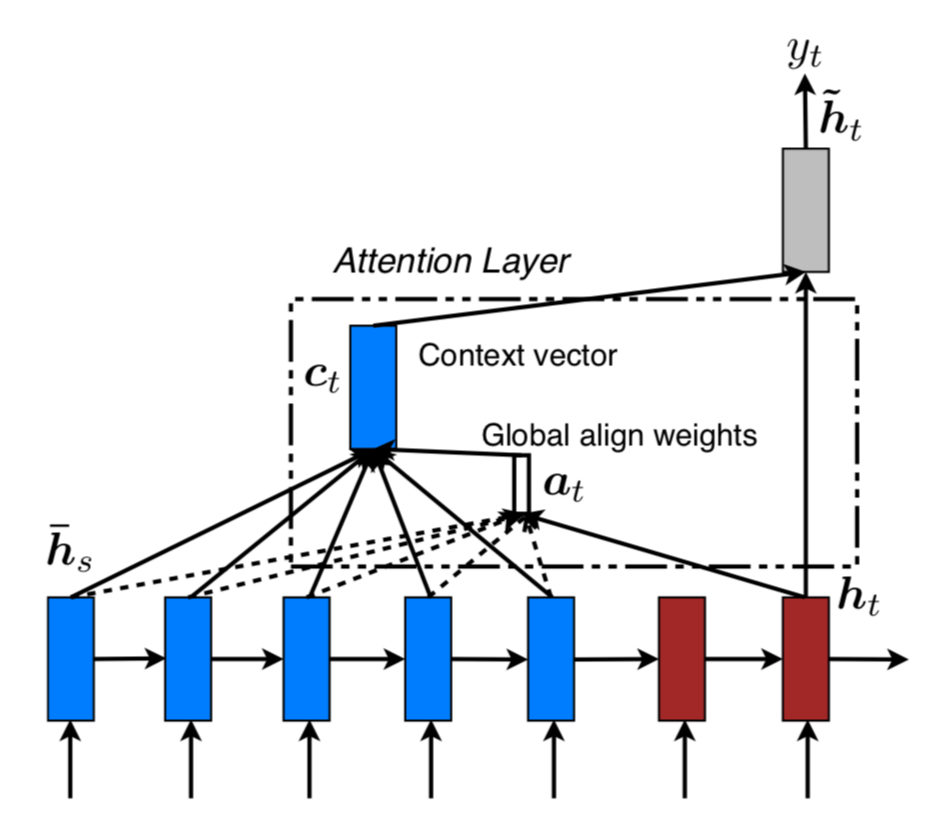
\includegraphics[width=0.6\hsize]{doc/figures/attention.png}
  \caption{Attention 機構の概略図 : 文献 \cite{attention} の図より引用}
  \label{fig:attention}
\end{figure}

\newpage
\changeindent{0cm}
\subsubsection{Transformer}
\changeindent{2cm}

Transformer \cite{transformer} は 他モデルで頻繁に用いられてきた RNN を用いずに
Attention 機構のみを基本構造とする Encoder-Decoder モデルである.
図 \ref{fig:transformer} にその概略図を示す.
Transformer のエンコーダおよびデコーダはそれぞれ Self-Attention を基本構造とする. Self-Attention とは, Attention 機構の特別な場合である.
Attention 機構は Query と Key-Value へのマッピングとして表現することが可能である.
通常 Query はデコーダからのターゲットを, Key-Valueはエンコーダからのソースを表す.
しかし Self-Attention は下層のすべての位置を参照することができシーケンスの依存関係を獲得できる.
%!数式の説明

\begin{figure}[!h]
  \centering
  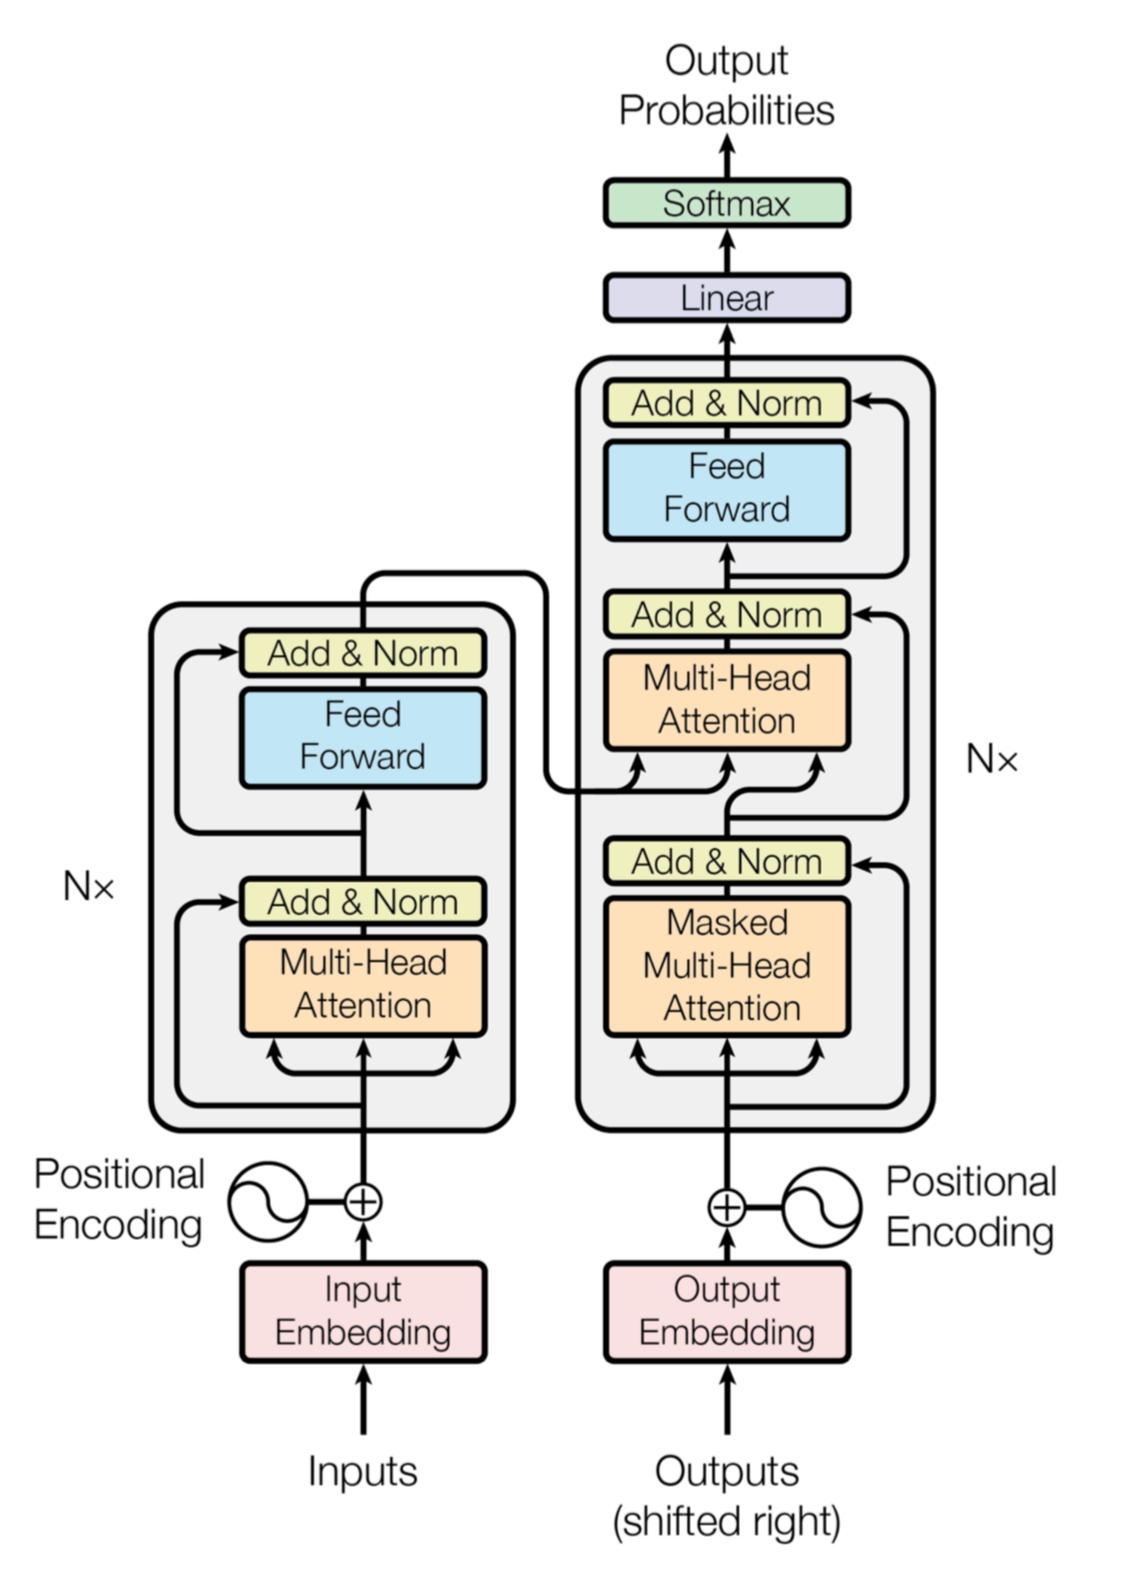
\includegraphics[width=0.5\hsize]{doc/figures/transformer.png}
  \caption{Transformer の概略図 : 文献 \cite{transformer} の図より引用}
  \label{fig:transformer}
\end{figure}

\newpage
\changeindent{0cm}
\subsubsection{BERT}
\changeindent{2cm}
Bidirectional Encoder Representations from Transformers (BERT) \cite{devlin2018bert} は, 2018 年に
Google が発表した言語モデルであり, 複数の双方向 Transformer に基づく汎用言語モデルである.
これまでの言語モデルは特定の学習タスクに対して 1 つのモデルを用いてきた. しかし BERT は
大規模コーパスに対して事前学習を施して, 各タスクに対してfine-tuning をすることで,
さまざまなタスクに柔軟に対応することができる. さらに, 以前はモデルごとに語彙を 1 から学習させるため, 非常に多くの時間とコストがかかって
いたが, BERT ではオープンソースで公開されている文脈を既に学習させた Pre-Training BERT モデルを使用することで短時間で学習ができる.

BERT の 事前学習では,周囲の単語からある単語を予測するMasked Language Model (MLM)
と 2 つ目の文章が 1 つ目の文章の次の文章であるかを予測する Next Sentence Prediction (NSP) によりモデルを学習する.

図 \ref{fig:bert_pre} に BERT の事前学習と fine-tuning の概略を示す.

\begin{figure}[h]
  \begin{center}
    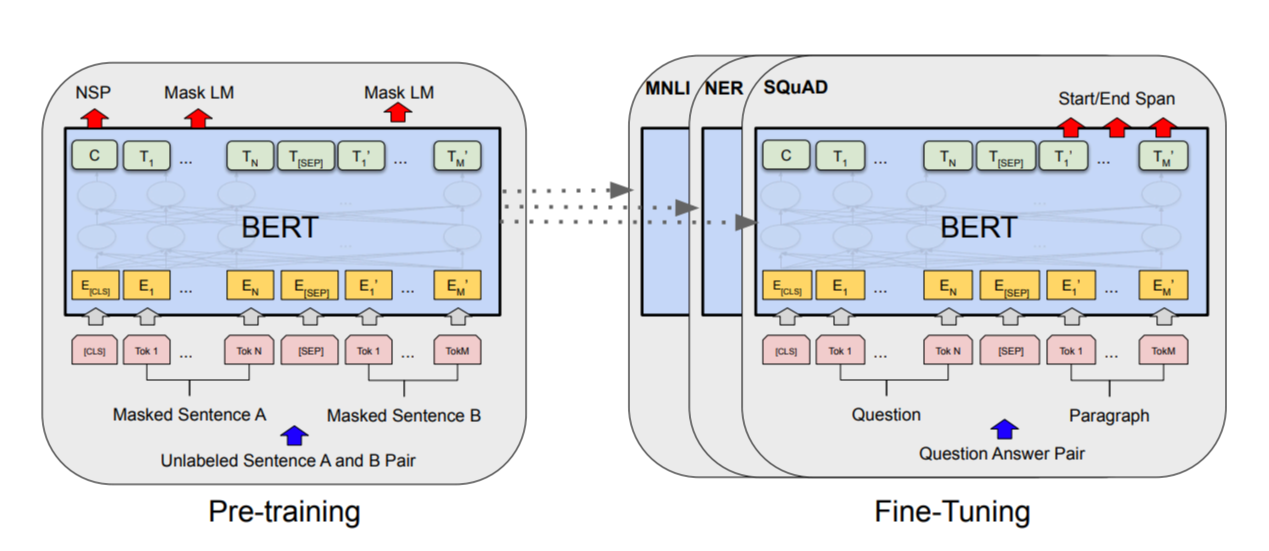
\includegraphics[width=0.8\hsize]{doc/figures/bert_pre.png}
    \caption{BERT の事前学習と fine-tuning の概略図 : 文献 \cite{devlin2018bert} の図より引用}
    \label{fig:bert_pre}
  \end{center}
\end{figure}

\newpage
\changeindent{0cm}
\subsection{画像処理に関する要素技術}
\changeindent{2cm}

画像処理に関する要素技術について説明する.

\changeindent{0cm}
\subsubsection{VGG}
\changeindent{2cm}

VGG \cite{brusilovsky:simonyan2014very} とは, ImageNet \cite{imagenet_cvpr09} と呼ばれる大規模
画像データセットで学習済みの畳み込みニューラル
ネットワーク (VGGNet) であり, 13 層の畳み込み層
と3 層の全結合層の合計 16 層からなる. 構成する層の数に応じて, VGG11 や VGG16 などと呼ばれることが多い. VGGNet は Oxford 大学に提案された手法であり, 2014 年の
画像認識大会で非常に好成績を収めたことからその
後のモデルアーキテクチャに広く取り入れられてい
る. あらかじめ学習が済んでいるモデルを転移学習
することで事前学習なしでも深いネットワークを学
習できる.

\changeindent{0cm}
\subsubsection{illustration2vec}
\changeindent{2cm}

illustration2vec \cite{i2v} は齋藤, 松井らが提案した VGG をベースとした画像のベクトル化手法であり, 画像リンク集サイトである Danbooru と Safebooru から 100 万枚のイラストを用いて学習した事前学習済みモデルが公開されている. illustration2vec が扱った問題として, イラストに対する画像認識の難しさがあり, VGG などの既存の画像認識モデルのほとんどが ImageNet などの実画像を評価対象にしており, アニメや漫画といったイラストに対して評価をしていなかった. illustration2vec はそれらの手法と比較して, より合理的なイラストのベクトル化が期待できる手法である. また, Danbooru と Safebooru でよく使われているタグを正解ラベルとして学習しているため, 簡単にイラストの特徴を検出でき, 大量の画像に対して類似画像を検索出来たり, 画像の意味における画像変換や応用例としてタグの特徴を満たす画像の生成などが可能となっている.
\newpage
illustration2vec では学習データを下記の要領で作成している.

\begin{enumerate}
  \item Danbooru と Safebooru から画像とメタデータを収集する.
  \item メタデータを 4 つのカテゴリに分類する.
        \begin{itemize}
          \item general : 一般的な属性 (例 : ``smile", ``short hair")
          \item copyright : 著作権名
          \item character : キャラクタ名
          \item rating : X レーティング (``safe", ``questionable", ``explicit")
        \end{itemize}
  \item general, copyright, character から最も使われている 512 個のタグをそれぞれ抽出する.
  \item 3 で抽出したタグと rating を連結させた 1539 個のタグをラベルとする.
\end{enumerate}

\changeindent{0cm}
\subsection{4 コマ漫画に関する従来研究}
\changeindent{2cm}

4 コマ漫画に関する研究としては,
4 コマにおける画像特徴が与える感情識別に関する研究 \cite{ueno-emotion2016} や
ストーリー理解過程の解析研究 \cite{ueno-oti2017},
4 コマ漫画ではないが既存漫画のデータを利用した
2 コマ漫画の生成に関する研究 \cite{jsai18mukaeyama} が報告されている.
また 4 コマ漫画の自動生成に関する研究 \cite{ueno:dcai2016}
や遺伝的アルゴリズムに基づく感性解析に
4 コマ漫画を用いた研究 \cite{GA4koma} もなされている.

また,ストーリーに関しては 4 コマ漫画の内容に踏み込んだ研究として,
コマの順序識別に関する研究 \cite{ueno2016estimation,jsai18fujino} が報告されている.
しかしながら手法,データセットともにまだ十分とは言えず,今後の発展が期待されている分野である.
